%%%%%%%%%%%%%%%%%%%%%%%%%%%%%%%%%%%%%%%%%%%%%%%%%%%%%%%%%%%%%%%%%%%%%%%%%%%%%%%%
\chapter{Разработка}
%%%%%%%%%%%%%%%%%%%%%%%%%%%%%%%%%%%%%%%%%%%%%%%%%%%%%%%%%%%%%%%%%%%%%%%%%%%%%%%%
\label{sec:development}

\section{Ограничения анализа в прототипа}
\label{sec:prototype-limits}

Как было сказано в разделе~\ref{sec:prototype-necessity}, для оценки
характеристик предложенного подхода для вывода типов параметров функций и его
применимости в среде разработки было решено разработать прототип и
проанализировать с его помощью ряд проектов с открытыми исходными текстами.

Прототипу требуется доступ к абстрактным синтаксическим деревьям (abstract
syntax tree --- AST) анализируемых модулей Python. В PyCharm и других средах
разработки на базе платформы
IntelliJ\footnote{\url{https://github.com/JetBrains/intellij-community}},
используется специальное высокоуровневое представление содержимого программы,
построенное поверх AST, называемое Program Structure Interface (PSI). 
В прототипе для построения AST используется модуль !ast! стандартной библиотеки
Python. Ввиду ограничений возможностей модуля !ast! и трудоемкости реализации на
базе его синтаксических деревьев многих видов анализа, имеющихся в PyCharm и
платформе IntelliJ для PSI, для прототипа был принят ряд допущений:

\begin{itemize} 
  \item Анализируемые программы не должны содержать синтаксических
  ошибок, поскольку, в отличие от парсера PyCharm, модуль !ast! не способен
  разбирать такие программы, выбрасывая исключение !SyntaxError!.

  \item Прототип не учитывает потока исполнения (flow-insensitive) и
    присваиваний и псевдонимов (aliases) внутри функций, собирая, например,
    атрибуты к которым происходит обращение во всех ветвях условных операторов,
    что потенциально сказывается на точности результатов.

  \item Для поиска атрибутов, определенных, в классах анализируются имена,
    определенные непосредственно в теле класса, т.е. методы и атрибуты
    класса, а также его конструктор --- метод !__init__!. В конструкторе
    анализируются только обращения к атрибутам значения переменной !self!. 
    При этом не учитывается, присваивается ли переменной с таким именем значение
    в теле функции или первый параметр конструктора назван иначе.

  \item Прототип имеет ограниченные возможности по разрешению имен в проектах, в
    частности не учитывает условных и локальных подключений модулей. В целом
    считается, что каждое имя внутри модуля объявлено только один раз.

  \item Прототип не повторяет имеющуюся функциональность PyCharm по выводу
    типов параметров функций. В частности он не учитывает типы
    аргументов по-умолчанию. По этой причине из списка параметров функции
    исключен первый параметр методов (!self!), не объявленных как !@classmethod!
    или !@staticmethod!, так как в PyCharm его значение всегда известно.

\end{itemize}


\nomenclature{AST}{Abstract Syntax Tree}
\nomenclature{PSI}{Program Structure Interface}

\section{Особенности реализации и основной цикл работы прототипа}
\label{sec:prototype-architecture}

Прототип не является интерактивным инструментом, как среда разработки, однако
для демонстрации применимости предложенного подхода в нем соблюдено требование
независимости индексации отдельных модулей программы: единственная информация,
содержащаяся в модуле и используемая в процессе индексации --- операторы
подключения других модулей, что используется для поиска проектных зависимостей,
однако это поведение можно отключить. Проектом в прототипе считается,
непосредственно указанный при запуске каталог, каталог, в котором находится
указанный модуль, либо первый родительский каталог где находится файл
конфигурации greentype.cfg.

Процесс индексации модулей в прототипе совмещен с поиском атрибутов параметров
функций. При индексации очередного модуля с исходными текстами происходит
сохранение в индекс четырех видов определений: !ModuleDef! --- определение
модуля программы, !ClassDef! --- определение класса, !FunctionDef! ---
определение функции и !ParameterDef! --- определение параметра функции. Для
каждого из них используется отдельный индекс, в котором нужное определение может
быть найдено по квалифицированному имени объекта. Например, параметр !x! метода
!func! класса !A! модуля !package.module! доступен в индексе параметров по имени
!package.module.A.func.x!. Одновременно с заполнением индекса классов
заполняется индекс атрибутов, определенных в классах, необходимый для
обеспечения быстродействия алгоритма подбора номинальных типов по структурным.

Индексы в прототипе не сохраняются на диске, как в PyCharm, а хранятся в
памяти во время работы прототипа и создаются заново при каждом его запуске. Роль
индексов выполняет стандартная коллекция !defaultdict!, представляющая собой
эффективную реализацию хэш-таблицы и предоставляющая независящее от числа
хранящихся в ней элементов (в отсутствие коллизий), близкое к константному
время поиска элемента по ключу. В качестве ключей во всех индексах используются
строки: квалифицированные имена для индексов модулей, классов, функций и
параметров и имена атрибутов для индекса классов, определяющих атрибут.

Всего в прототипе используется пять индексов, состав и назначение которых
перечислены в таблице \ref{tab:indexes-ref} в приложении~\ref{app:tables}.

Вывод типов параметров функций в прототипе осуществляется не в отдельности для
каждого из них, как происходило бы в среде разработки, а для всех параметров
всех функций в проекте сразу.


Для индексации скомпилированных модулей, входящих в стандартную библиотеку, в
первую очередь модуля
!builtins!\footnote{\url{https://docs.python.org/3.4/library/builtins.html}},
где определены стандартные коллекции, такие как !list!, !tuple!, !dict! и !set!,
используются имеющиеся в языке механизмы интроспекции, тогда как в PyCharm
такие стандартные классы и функции описываются при помощи модулей-заглушек.
Изначально таким образом индексируются только некоторые модули стандартной
библиотеки, однако имеется возможность указать в настройках для конкретного
проекта дополнительные модули, которые будут проанализированы рефлексивно.

Для поиска импортируемых модулей, например, для поиска определений базовых
классов используется стандартный путь интерпретатора Python !sys.path!, а также пути
указанные в настройках прототипа (либо через файл конфигурации, либо через
аргументы командной строки). Это необходимо для того, чтобы проектные
зависимости также учитывались в процессе анализа.

В целом порядок работы прототипа, описанный в методе !GreenTypeAnalyzer.main()! 
выглядит следующим образом:

\begin{enumerate}
    \item Разбор аргументов командной строки, поиск и чтение проектного файла
      конфигурации.

    \item Рефлексивная индексация скомпилированных модулей (метод
      !GreenTypeAnalyzer.index_builtins()!).

    \item Индексация всего проекта, начиная с указанного модуля или каталога 
      (метод !GreenTypeAnalyzer.index_project()!).
      Включаемые и исключаемые из процесса индексации файлы и каталоги, а также
      пути для поиска модулей настраиваются. 

    \item Подбор для всех параметров в проекте подходящих классов (метод
      !GreenTypeAnalyzer.infer_parameter_types()!).

    \item Формирование отчета (метод !GreenTypeAnalyzer.statistics_report()!),
      который затем выводится на консоль или записывается в файл. Отчет может
      быть представлен в неструктурированном и более удобном для чтения
      текстовом виде либо в формате JSON.

\end{enumerate}

\section{Описание классов прототипа}
\label{sec:classes-description}

Подробная диаграмма классов, используемых в прототипе, приведена на
 рисунке~\ref{fig:classes-diag} приложении~\ref{app:diagrams}.

Рассмотрим подробнее назначение некоторых из приведенных на диаграмме компонентов.

\begin{description}
  \item[GreenTypeAnalyzer] \hfill \\
    Данный класс является центральным компонентом системы. Он хранит индексы,
    инициирует процесс индексации модулей, отвечает за разрешение имен и подбор
    номинальных типов для параметров. Процедура индексации модуля запускается
    вызовом метода !index_module!, который принимает как квалифицированное имя,
    так и путь к файлу с исходными текстами. Перед запуском индексации
    происходит разрешение пути к модулю или его имени (в зависимости от того, что
    не указано) и проверятся наличие модуля в индексе. Если модуль еще не был
    разобран, создается объект класса !SourceModuleIndexer!, который отвечает
    непосредственно за обход AST конкретного модуля и извлечение из него
    определений классов, функций и параметров, необходимых для процедуры вывода
    типов.

  \item[SourceModuleIndexer] \hfill \\ !SourceModuleIndexer! наследуется от
    стандартного класса !ast.NodeVisitor!, представляющего стандартный
    \emph{визитор} (\emph{visitor}) для AST, которое возвращает функция
    !ast.parse!. Он расширяет функциональность базового класса, храня, в
    частности, стек
    \emph{блоков}\footnote{\url{https://docs.python.org/3.4/reference/executionmodel.html\#naming-and-binding}},
    задающих пространства имен в Python: модули, классы и функции. Стек
    используются для того, чтобы определить \emph{квалифицированное имя}
    (\emph{qualified name}) объекта в программе.  Как только в процессе
    рекурсивного обхода всех узлов в AST, встречается определение модуля (один
    раз в начале), класса или функции, вызывается один из методов
    !module_discovered!, !class_discovered! или !function_discovered!
    соответственно, которым передается текущий узел в AST. Каждый из этих
    методов при необходимости обходит поддерево от узла дальше и возвращает
    нужный объект, описывыющий определение в программе (наследники класса
    !Definition!), которое кладется на стек. Дополнительно этот объект
    регистрируется в одном из индексов
    (функции !register_module!, !register_class! и !register_function!).
    Индексация запускается вызовом метода !run!, который возвращает описание
    для проиндексированного модуля. Взаимодействие классов !GreenTypeAnalyzer! и
    !SourceModuleIndexer! на примере разбора определения класса
    проиллюстрировано на рисунке~\ref{fig:indexing-diag}.
    % Шаблон проектирования \emph{визитор}! (\emph{Visitor}) является
    % стандартным способом обхода древовидных структур с различными типами узлов
    % в объектно-ориентированных языках. Интересно, что тогда как статически
    % типизированных языках принцип его работы основан на 

  \begin{figure}
  \begin{center}
      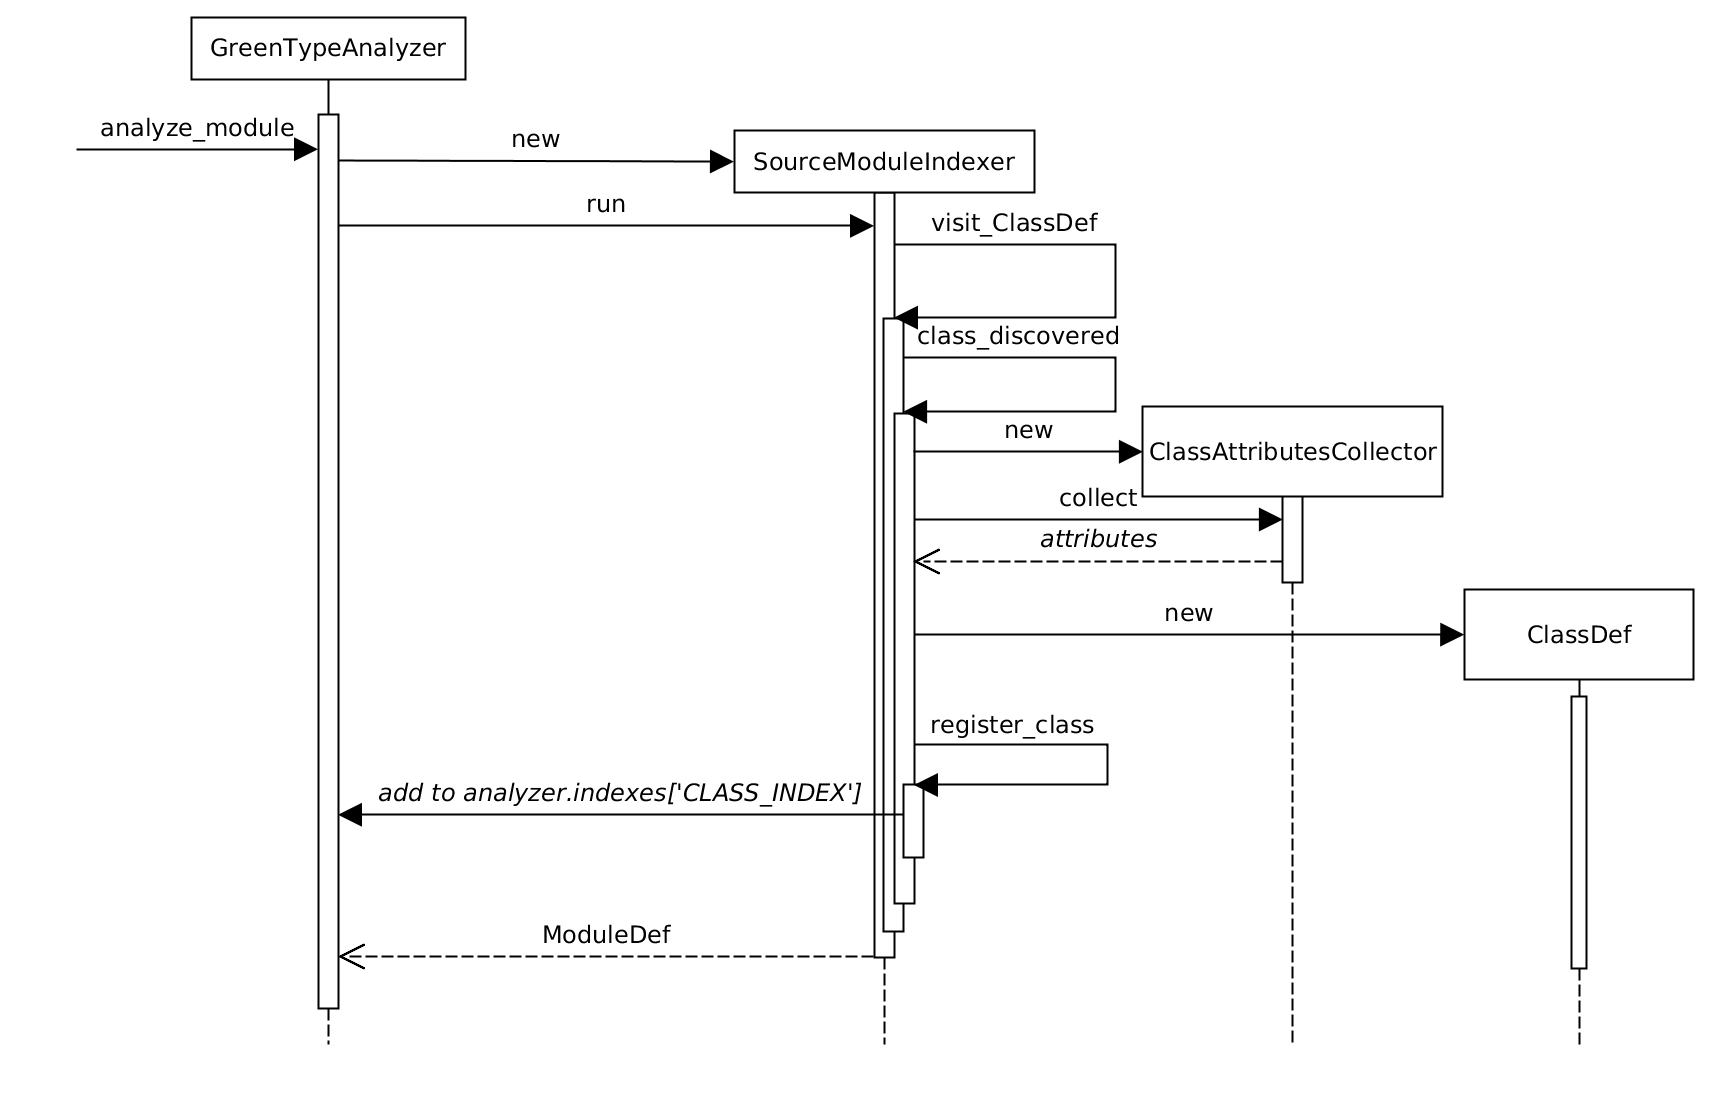
\includegraphics[width=\textwidth]{fig/indexing-diag.png}
  \end{center}
  \caption{Диаграмма процесса индексации модуля}
  \label{fig:indexing-diag}
  \end{figure}

  \item[Config] \hfill \\
    Настройки для анализатора могут быть указаны, как через аргументы командной
    строки (для чего используется стандартный модуль !argparse!), так и через
    конфигурационный файл !greentype.cfg! (на данный момент только пути поиска
    модулей --- !source-roots!) , что было необходимо для анализа
    проектов в режиме сбора статистики (подробнее в разделе
    \ref[sec:statistics-collecting]). Для того чтобы убрать из
    !GreenTypeAnalyzer! логику разбора аргументов и чтения файла конфигурации, а
    также сделать добавление новых настроек проще, его настройки представлены
    экземпляром класса !Config!. Он имеет такой же интерфейс, что и стандартная
    коллекция !dict!, однако также включает вспомогательные методы
    !update_from_object! и !update_from_cfg_file!. Пример файла формата файла
    конфигурации приведен в листинге~\ref{lst:config-file-sample}. Все настройки
    анализатора, их назначение и формат соответствующих аргументов командной
    строки приведены на таблице~ref{tab:config-ref}.
  \item[StatisticsReport] \hfill \\
    Первоначально различная статистика в проекте, например, суммарное количество
    проиндексированных модулей, классов, функций и параметров, количество
    параметров, для которых был найден только один подходящий класс
    (!single_type_parameters!) или количество параметров, для которых нашлось
    несколько классов или вообще ни одного , подсчитывалась и отображалась в
    консоли в неструктурированном виде. Однако это оказалось неудобно для
    последующей оценки полученных данных и подсчета статистики. Поэтому подсчет
    и форматирование результатов статистики были вынесены в отдельный класс
    !StatisticsReport!. Он имеет ряд вспомогательных методов для анализа
    содержимого индексов (например,!undefined_parameters!  или
    !scattered_type_parameters!), а полученные результаты могут быть
    представлены в виде текстового отчета (!format_text!) или JSON
    (!format_json!). 

  
\end{description}

\begin{lstlisting}[
  language=,
  label={lst:config-file-sample},
  caption={Пример формата файла конфигурации}
]
[greentype]

project_name = config-test
source_roots = src1:src2
some_param = 42
exclude = excluded:excluded/included/excluded_explicitly.py
include = excluded/included
builtins = audioop:ssl
\end{lstlisting}

\begin{table}[H]
  \small
  \caption{Параметры конфигурации анализатора.}
  \label{tab:config-ref}
  \begin{tabularx}{\textwidth}{ |X|X|X| }
    \hline
    Название & Аргумент командной строки & Значение \\
    \hline
    \texttt{TARGET\_NAME} & \texttt{-t}, \texttt{--target} &  Фильтрация
    объектов, отображаемых в статистике по префиксу квалифицированного имени.
    \\ \hline

    \texttt{VERBOSE} & \texttt{-v}, \texttt{--verbose} & Режим подробного
    (verbose) вывода, включающего сообщения логгирования с уровнем
    \texttt{DEBUG} и выше.
    \\ \hline

    \texttt{FOLLOW\_IMPORTS} & \texttt{-L}, \texttt{--follow-imports} & 
    Индексация импортируемых модулей (обход модулей проекта в DFS порядке).
    \\ \hline

    \texttt{ANALYZE\_BUILTINS} & \texttt{-B}, \texttt{--no-builtins} &
    Рефлексивно анализировать встроенные (скомпилированные) модули стандартной
    библиотеки.
    \\ \hline

    \texttt{BUILTINS} & --- & Список встроенных модулей для рефлексивной
    индексации.
    \\ \hline
    
    \texttt{SOURCE\_ROOTS} & \texttt{--src-roots} & Корневые каталоги проекта.
    Необходимы для поиска модулей по имени.  
    \\ \hline

    \texttt{TARGET\_PATH} & обязательный аргумент & Начальный каталог или
    конкретный модуль, с которого начинается анализ проекта.
    \\ \hline

  \end{tabularx}
\end{table}

\section{Сбор статистики}
\label{sec:statistics-collecting}

Для оценки эффективности предложенного метода вывода типов параметров функций,
прототип собирает статистику по результатам анализа. Измеряемые метрики включают
в себя:

\begin{enumerate}
  \item Количество проиндексированных модулей, классов, функций и параметров в
    проекте (без зависимостей и стандартной библиотеки) и в целом.

  \item Параметры функций, содержащие максимальное число уникальных атрибутов, к
    которым происходило обращение. В отчет также могут быть включены примеры
    параметров с наибольшим числом обращений к атрибутам.

  \item Параметры функций, к атрибутам которых не происходило обращений в теле
    функции (\emph{attributeless parameters}). Для них также
    собирается информация о том, какие из них тем не менее использовались в
    качестве возвращаемого значения функции (!ParameterDef.returned!), операнда
    в арифметическом выражении (!ParameterDef.used_as_operand!) или аргумента
    другой функции (!ParameterDef.used_as_argument!).

  \item Параметры функций, к атрибутам которых происходило обращение, но для
    которых тем не менее не было найдено ни одного подходящего класса
    (\emph{undefined parameters}).

  \item Параметры функций, к атрибутам которых происходило обращение, и для
    которых был найден только один подходящий класс (\emph{exact type parameters}).

  \item Параметры функций, к атрибутам которых происходило обращение, но для
    которых было найдено более одного подходящего класса (\emph{scattered type
      parameters}).

\end{enumerate}

Все группы параметров для чистоты измерений включают только параметры функций
проекта. В результаты измерений также можно включить примеры параметров каждой из
групп. Статистика собранная для ряда публично доступных проектов на Python,
обсуждается в разделе~\ref{sec:projects-analysis}.

\section{Модульное тестирование}
\label{sec:unit-testing}

Модульное тестирование созданного прототипа осуществлялось при помощи библиотеки
pytest\footnote{\url{http://pytest.org/latest/}}.  Тестируемые функции прототипа
включают:

\begin{itemize}
    \item индексацию модулей
    \item поиск определений классов
    \item поиск и чтение конфигурации проекта
    \item подбор для параметров функций классов, определенных в самом проекте и
      стандартной библиотеке, в том числе проиндексированных рефлексивно
    \item сбор статистики и форматирование отчета
    \item подбор наиболее общих из подходящих по структуре классов в случае
      множественного наследования и ромбовидных иерархий классов
    \item функциональность различных вспомогательных функций для работы с
      путями и строками, использованных в прототипе
\end{itemize}

Всего в проекте 30 модульных текстов. Пример модульного теста для проверки
индексации проекта с настройками включения/исключения путей приведен в
листинге~\ref{lst:unit-test-example}.

\begin{lstlisting}[
  caption={Пример модульного теста},
  label={lst:unit-test-example}
]

def test_module_exclusion():
    analyzer = conftest.TestAnalyzer('module_exclusion')
    analyzer.config['EXCLUDE'] = ['excluded']
    analyzer.config['INCLUDE'] = ['excluded/included']

    analyzer.index_project()

    assert 'main' in analyzer.indexes['MODULE_INDEX']
    assert 'excluded' not in analyzer.indexes['MODULE_INDEX']
    assert 'excluded.module' not in analyzer.indexes['MODULE_INDEX']
    assert 'excluded.included' in analyzer.indexes['MODULE_INDEX']
    assert 'excluded.included.module' in analyzer.indexes['MODULE_INDEX']

\end{lstlisting}
